\documentclass[12pt]{article}
\usepackage{graphicx}
\usepackage{amssymb}
\usepackage{epstopdf}
\usepackage{amsmath}
\usepackage{multicol}
\usepackage{tcolorbox}
\usepackage{geometry}
\usepackage{enumitem}
\usepackage{fancyhdr}

\DeclareGraphicsRule{.tif}{png}{.png}{`convert #1 `dirname #1`/`basename #1 .tif`.png}

\textwidth = 6.5 in
\textheight = 9 in
\oddsidemargin = 0.0 in
\evensidemargin = 0.0 in
\topmargin = -23pt
\headheight = 0.0 in
\headsep = 0.0 in
\parskip = 0.2in
\parindent = 0.0in
\pagestyle{fancy}
\pagenumbering{gobble}

\newtheorem{theorem}{Theorem}
\newtheorem{corollary}[theorem]{Corollary}
\newtheorem{definition}{Definition}
%\includegraphics [height=50mm, width=50mm]{PathInt.jpg}
\title{Title} 

\begin{document}
%INSTRUCTOR NOTES
%No warm-up on quiz days. If wanted, today's warm-up would be solving equations.
 Name:
 \begin{center}\large{2.6 Differentiability}\end{center}

\begin{tcolorbox}
A function $f$ is \textit{differentiable} at $x=a$ if...
\vspace{20mm}
\end{tcolorbox}

\begin{enumerate}

\item Warm-up:
	\begin{enumerate}
	\item Sketch a function that is continuous but not differentiable at $x=0$, or explain why it's not possible.
	\vfill
	\item Sketch a function that is differentiable but not continuous at $x=0$, or explain why it's not possible.
	\vfill
	\end{enumerate}
	
\item The function $f(x)$ is shown below:\\
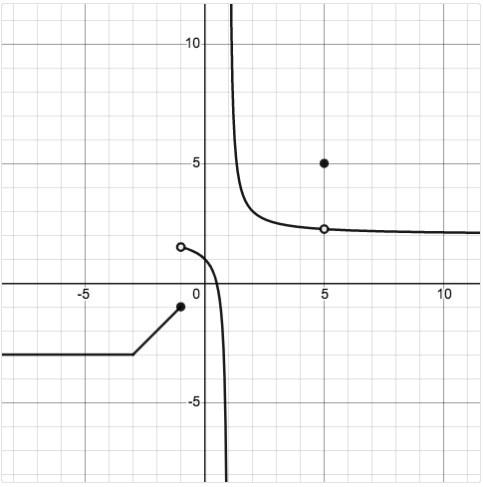
\includegraphics[scale=.6]{2_6_g1}
	\begin{enumerate}
	\item At what values is $f(x)$ not continuous?
	\item At what values is $f(x)$ not differentiable?
	\item BONUS: Sketch a graph of $f'(x)$.
	\end{enumerate}

\newpage
~
\rhead{2.6 Differentiability }

\item Let $f(x)$ be given by:\\
	$f(x) = \begin{cases} 
				
     				 kx+b & x<2 \\
     				 x^2-2 & x \geq 2 \\
  				\end{cases} $	

Find a values of $k$ and $b$ so that $f$ is continuous and differentiable at $x=2$.

	\vfill



\item A magnetic field, $B$, is given as a function of the distance, $r$, from the center of a wire as follows:
	\[B= \begin{cases} 
     				 \frac{r}{r_0}B_0&\text{for }r\leq r_0 \\
     				 \frac{r_0}{r}B_0&\text{for }r> r_0 \\
  				\end{cases} \]
	\begin{enumerate}
	\item Is $B$ continuous at $r_0$? Explain.
	\vfill
	\item Is $B$ differentiable at $r_0$? Explain.
	\vfill
	\end{enumerate}



\end{enumerate}
\end{document} 
A company charges a flat rate of \$500 to rent up to 100 chairs and every additional chair costs \$4. Draw a graph and find a formula for the cost $C$ as a function of $n$, the number of chairs rented.\\
%%%%%%%%%
\begin{tcolorbox}
\textbf{Warm-up: } Solve the following equations for $t$.
\begin{multicols}{2}
\begin{enumerate}
\item $(t+1)^2=9$
\item $tx+x^2=5$
\end{enumerate}
\end{multicols}
\end{tcolorbox}

MINIPAGE
\noindent\begin{minipage}{0.3\textwidth}% adapt widths of minipages to your needs
try 1
\end{minipage}%
\hspace{40mm}
\begin{minipage}{0.6\textwidth}
a) $f'(2)=$\\\

b) $f'(4)=$\\

c) $f'(6)=$\\

d) $f'(7)=$\\

e) $f'(8)=$
\end{minipage}
